% !TEX root = ../dg.tex

\section{Geodesics}
\label{sec:geodesics}

Geodesics are generalizations of straight lines to Riemannian manifolds.\footnote{As mentioned briefly at the end of \Cref{sec:connections}, we can define geodesics for any affine connection, so geodesics are really generalizations of straight lines to manifolds-with-connections, but we're only going to develop the theory here for the Levi-Civita connection.} Typically we think of straight lines in the plane or in space as \emph{shortest paths}, but this is actually the wrong notion to generalize. Not because shortest paths won't be geodesics, but because not all geodesics are shortest paths.

\begin{example}
	The geodesics on the round sphere will turn out to be arcs of great circles. Of course, the shortest path between two points will be an arc of a great circle, but we can get another geodesic between any two non-antipodal points by going the long way around: instead of traveling from Ecuador to Kenya by flying east along the equator over South America and the Atlantic Ocean, head west over the Pacific Ocean, Indonesia, and the Indian Ocean. The latter route is still a geodesic, but certainly not the shortest path.
\end{example}

Instead, the right notion to generalize is that straight lines are (no surprise) \emph{straightest paths}. We can see this in terms of formulas by taking a constant-speed parametrization of a straight line, something like $\alpha(t) = p + tv$, for $p,v \in \R^n$. Then $\alpha'(t) = v$ is constant, and hence $\alpha''(t) = 0$. The equation $\alpha''(t) = 0$ is going to generalize to the so-called \emph{geodesic equation}.

\begin{definition}\label{def:geodesic}
	Let $(M,g)$ be a Riemannian manifold and let $\nabla$ be the Levi-Civita connection on $M$. A curve $\gamma \from I \to M$ is a \emph{geodesic} if 
	\begin{equation} \label{eq:geodesic}
		\frac{D}{dt} \gamma'(t) = 0 
	\end{equation}
	for all $t \in I$. The equation \eqref{eq:geodesic} is the \emph{geodesic equation}.
\end{definition}

\begin{remark}
	A geodesic is automatically traversed at constant speed:
	\[
		\frac{d}{dt} g_{\gamma(t)} (\gamma'(t),\gamma'(t)) = 2 g_{\gamma(t)} \left(\frac{D}{dt} \gamma'(t), \gamma'(t)\right) = 0
	\]
	by \Cref{ex:compatibility and covariant differentiation}. 
\end{remark}

Let's work out what the geodesic equation~\eqref{eq:geodesic} looks like in local coordinates. So work in a local coordinate chart on $M$. Suppose $\gamma(t) = (x_1(t),\dots , x_n(t))$ is a curve and $W(t) = \sum_j w_j(t) \frac{\partial}{\partial x_j}$ is a vector field along $\gamma$. We saw in~\eqref{eq:connection local coords} that 
\[
	\frac{DW}{dt} = \sum_{i,j,k}\left( w_k'(t) + \Gamma_{ij}^k x_i'(t) w_j(t)\right)\frac{\partial}{\partial x_k}.
\]
So if
\[
	W(t) = \gamma'(t) = \sum_j x_j'(t) \frac{\partial}{\partial x_j},
\]
then we have
\[
	\frac{D}{dt}\gamma'(t) = \sum_{i,j,k} \left(x_k''(t) + \Gamma_{ij}^k x_i'(t)x_j'(t)\right)\frac{\partial}{\partial x_k}.
\]
Then $\gamma$ is a geodesic if and only if the above is zero, which means all the coefficients must be zero:
\begin{equation}\label{eq:geodesic in coords}
	x_k''(t) + \sum_{i,j} \Gamma_{ij}^k x_i'(t)x_j'(t) = 0 \quad \text{for } k = 1, \dots , n,
\end{equation}
which is a system of $n$ second-order ODEs on a coordinate neighborhood of $M$.

\begin{example}
	Let's figure out the geodesic equation on $\Aff^+(\R) \cong H = \{(x,y) \in \R^2 : y > 0\}$. We saw in \Cref{ex:affine hyperbolic metric} that the metric is given by $g_{11} = \frac{1}{y_2} = g_{22}$, $g_{12} = 0$, and we worked out the Levi-Civita connection in \Cref{ex:hyperbolic plane connection}. Specifically,~\eqref{eq:hyperbolic plane Christoffel} implies that
	\begin{align*}
		\Gamma_{11}^1 & = 0 & \Gamma_{12}^1 = \Gamma_{21}^1 & = -\frac{1}{y} &  \Gamma_{22}^1 & = 0 \\
		\Gamma_{11}^2 & = \frac{1}{y} & \Gamma_{12}^2 = \Gamma_{21}^2 & = 0 & \Gamma_{22}^2 & = -\frac{1}{y}.
	\end{align*}
	
	Therefore,~\eqref{eq:geodesic in coords} becomes
	\begin{align}\label{eq:hyperbolic geodesic coords}
		x''(t) - \frac{2}{y} x'(t)y'(t) & = 0 \\
		y''(t) + \frac{1}{y}((x'(t))^2 - (y'(t))^2) & = 0. \nonumber
	\end{align}
	On vertical rays, $x(t) = \text{constant}$, so the first equation is satisfied and the second reduces to $y''= \frac{(y')^2}{y}$, which has solution $y(t) = c_1 e^{c_2t}$. So the vertical rays parametrized as $\gamma(t) = (x_0,c_1e^{c_2t})$ are geodesics. We can eliminate the constants by deciding that we want $\gamma(0) = (a,1)$, which implies $c_1 = 1$, and that we want $\gamma'(0) = (0,1)$:
	\[
		(0,1) = \gamma'(0) = (0,c_2)
	\]
	so $c_2 = 1$. That is, $\gamma(t) = (a,e^t)$ is a geodesic in $H$ for any $a \in \R$.
	
	As for the other geodesics, note that $\frac{dy}{dx} = \frac{y'}{x'}$, which we can differentiate as follows:
	\[
		\frac{d^2 y}{dx^2} = \frac{d}{dx} \left( \frac{y'}{x'} \right) =\frac{x'y'' - y'x''}{(x')^2} \frac{1}{x'}
	\]
	since $\frac{df}{dx} = \frac{df}{dt} \frac{dt}{dx} = \frac{\frac{df}{dt}}{\frac{dx}{dt}}$. If we assume our curve $\gamma(t) = (x(t),y(t))$ is a geodesic, we can substitute in $x'' = \frac{2}{y} x'y'$ and $y'' = \frac{1}{y} ((y')^2 - (x')^2)$ from~\eqref{eq:hyperbolic geodesic coords}:
	\begin{align*}
		\frac{d^2 y}{dx^2} & = \frac{1}{(x')^3}\left(\frac{x'}{y}((y')^2-(x')^2) - \frac{2}{y}x'(y')^2\right) \\
		& = \frac{1}{(x')^3}\frac{1}{y}\left(-(x')^3 - x'(y')^2\right) \\
		& = -\frac{1}{y} \left(1 + \frac{(y')^2}{(x')^2}\right) \\
		& = -\frac{1}{y} \left(1 + \left( \frac{dy}{dx}\right)^2\right).
	\end{align*}
	(Note that we're implicitly assuming $x' \neq 0$ here, which is why we dealt with the $x(t) = \text{constant}$ case separately.)
	
	In other words,
	\[
		-1 = y \frac{d^2y}{dx^2} + \left(\frac{dy}{dx}\right)^2 = \frac{d}{dx} \left( y \frac{dy}{dx} \right)
	\]
	on a geodesic. Integrating twice gives the solution
	\[
		x^2 + y^2 = ax + b,
	\]
	which is the semi-circle of radius $\sqrt{b+\frac{a^2}{4}}$ centered at the point $(a/2,0)$.
	
	In other words, we've proved that the geodesics in $H$ are the vertical rays and the semi-circles centered at points on the $x$-axis, as claimed in \Cref{ex:hyperbolic plane}.
	
	\begin{figure}[htbp]
		\centering
			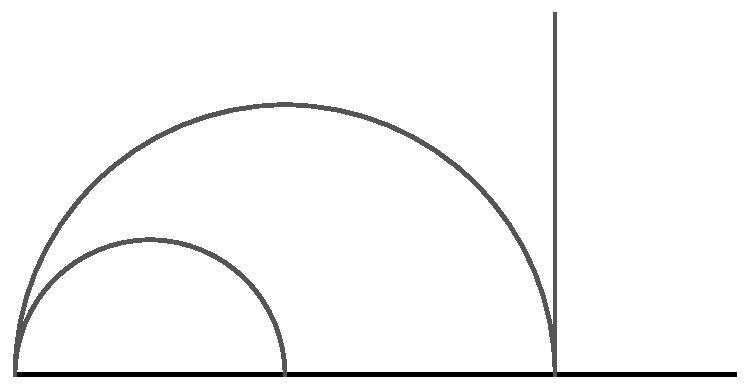
\includegraphics[height=1.5in]{hyperbolicgeodesics}
		\caption{Some geodesics in $H$.}
		\alttext{The upper half-plane, shown with three curves: a vertical line and two semi-circles centered at points on the $x$-axis.}
		\label{fig:hyperbolicgeodesics2}
	\end{figure}
\end{example}

If we want to convert~\eqref{eq:geodesic in coords} to a system of $2n$ first-order ODEs, we need to pass to the tangent bundle $TM$. Recall that
\[
	TM := \bigsqcup_{p \in M} T_pM.
\]
Suppose $p \in M$ lies in a coordinate chart $(U,\phi)$. If $v \in T_p M$, then $v = \sum_i y_i \frac{\partial}{\partial x_i}$ for some $y_1, \dots , y_n$; then $(x_1, \dots , x_n, y_1, \dots , y_n)$ give local coordinates on $T(\phi(U)) \cong U \times \R^n$; continuing down this path gives the proof of \Cref{ex:tangent bundle manifold}.

In any case, the curve $t \mapsto \gamma(t)$ in $M$ determines a curve $t \mapsto (\gamma(t),\gamma'(t))$ in $TM$ and, if $\gamma$ is a geodesic, then in a local coordinate neighborhood $T(\phi(U))$ this curve satisfies the first-order system
\begin{align}\label{eq:first-order geodesic}
	x_k'(t) & = y_k(t) \\
	y_k'(t) & = -\sum_{i,j} \Gamma_{ij}^k y_i(t)y_j(t) \nonumber
\end{align}
for all $k =1 , \dots , n$.

By the usual existence and uniqueness theorems for solutions to ODEs, it will follow that, for any $p \in M$ and any $v \in T_pM$ (or, alternatively, any $(p,v) \in TM$), there will be a geodesic $\gamma \from (-\epsilon,\epsilon) \to M$ with $\gamma(0) = p$ and $\gamma'(0) = v$ and that any other solution will agree with $\gamma$ on the overlap of their domains. We can package this up into a single vector field on $TM$ which we will call the geodesic field.

\begin{theorem}\label{thm:geodesic field}
	Let $(M,g)$ be a Riemannian manifold. Then there is a unique smooth vector field $G$ on $TM$ whose integral curves are of the form $t \mapsto (\gamma(t), \gamma'(t))$, where $\gamma$ is a geodesic on $M$.
\end{theorem}

Recall from \Cref{def:integral curve} that an integral curve of a vector field is one whose velocity agrees with the vector field at every point along the curve.

\begin{proof}
	Suppose such a $G$ exists. Then the trajectories of $G$ must be given by $t \mapsto (\gamma(t), \gamma'(t))$, which must solve the system~\eqref{eq:first-order geodesic} in local coordinates. By uniqueness of the trajectories of such a system, $G$ must be unique.
	
	On the other hand, to prove that such a $G$ exists, we can simply define it in coordinates by the system~\eqref{eq:first-order geodesic}.
\end{proof}

\begin{definition}\label{def:geodesic field}
	The vector field $G \in \mathfrak{X}(TM)$ defined in \Cref{thm:geodesic field} is called the \emph{geodesic field} on $TM$ and its local flow is called the \emph{geodesic flow} on $TM$.
\end{definition}

\begin{example}
	Let $M = S^1$ with its usual metric, namely $g_\theta \left( \frac{\partial}{\partial \theta},\frac{\partial}{\partial \theta}\right) = 1$. It's straightforward to check using~\eqref{eq:levi-civita formula} that 
	\[
		\nabla_{\frac{\partial}{\partial \theta}}\frac{\partial}{\partial \theta} = 0.
	\]
	So then the system~\eqref{eq:first-order geodesic} on $TS^1 = S^1 \times \R$ with coordinates $(\theta, y)$ reduces to
	\begin{align*}
		\theta'(t) & = y(t) \\
		y'(t) & = 0.
	\end{align*}
	Solutions are of the form $(\gamma(t),\gamma'(t)) = (c_1 + c_2 t,c_2)$, so when we require $\gamma(0) = \theta_0$ and $\gamma'(0) = y_0 \frac{\partial}{\partial \theta} \in T_{\theta_0}S^1$, we get $\gamma(t) = \theta_0 + y_0 t$. These curves are trajectories of the field
	\[
		G(\theta,y) = (y,0)
	\]
	on the cylinder, as shown in \Cref{fig:circle geodesic field}. This makes sense: geodesics go around the circle at constant speed, and this speed is determined by the initial velocity, which corresponds to height on the cylinder in this picture.
	\begin{figure}[htbp]
		\centering
			\includegraphics[height=1.5in]{circlegeodesicfield}
		\caption{The geodesic field on $TS^1 = S^1 \times \R$. The zero section $\{(\theta,0)\} \cong S^1$ is shown in dark blue.}
		\alttext{A vector field on the cylinder which points horizontally: counterclockwise above the equatorial circle on the cylinder, and clockwise below the equatorial circle. The lengths of the vectors is proportional to their height above the equatorial circle.}
		\label{fig:circle geodesic field}
	\end{figure}
\end{example}

\begin{example}
	Let $M = S^2$ with the Riemannian metric induced by the Euclidean metric on $\R^3$. We'll work locally in spherical coordinates $(\phi,\theta) \mapsto (\cos \theta \sin \phi, \sin \theta \sin \phi, \cos \phi)$. 
	
	\begin{exercise}
		Show that in these coordinates,
		\begin{align*}
			\Gamma_{11}^1 & = 0 & \Gamma_{12}^1 = \Gamma_{21}^1 & = 0 &  \Gamma_{22}^1 & = -\sin \phi \cos \phi \\
			\Gamma_{11}^2 & = 0 & \Gamma_{12}^2 = \Gamma_{21}^2 & = \cot \phi & \Gamma_{22}^2 & = 0.
		\end{align*}
	\end{exercise}
	
	Therefore, in the coordinates $(\phi, \theta, y, z)$ on $TS^2$,~\eqref{eq:first-order geodesic} becomes
	\begin{align*}
		\phi' & = y \\
		\theta' & = z \\
		y' & = (\sin \phi) (\cos \phi) z^2 \\
		z' & = - (\cot \phi) y z.
	\end{align*}
	If we want the geodesic through $(\phi_0,\theta_0) \in S^2$ with initial velocity $v \in T_{(\phi_0,\theta_0)}S^2$, then this gives a well-defined initial value problem.
	
	It's not so clear to me how to solve this problem analytically, but we could certainly solve it numerically for any desired $\phi_0,\theta_0,v$, and then the velocities of these geodesics would give the geodesic field $G$ on $TS^2$ (which is a nontrivial bundle: $TS^2 \not\cong S^2 \times \R^2$).
\end{example}

The existence of the geodesic flow follows from \Cref{prop:local flow}. More precisely, if $U \subset M$ is an open set and $\epsilon > 0$, we'll use the notation
\[
	TU_\epsilon := \{(p,v) \in TU : |v|<\epsilon\}.
\]
Then applying \Cref{prop:local flow} to the geodesic field $G$ on $TM$ at the point $(p,0) \in TM$ yields:
\begin{proposition}\label{prop:geodesic flow}
	Let $M$ be a Riemannian manifold and let $p \in M$. There is an open set $U$ containing $p$, real numbers $\delta,\epsilon > 0$, and a smooth map $\phi \from (-\delta, \delta) \times TU_\epsilon \to TU$ so that $t \mapsto \phi(t,q,v)$ is the unique trajectory of the geodesic field $G$ with $\phi(0,q,v) = (q,v)$ for all $(q,v) \in TU_\epsilon$.
\end{proposition}

Composing the local flow $\phi$ with the projection $\pi \from TM \to M$ yields the map $\gamma = \pi \circ \phi$ which satisfies:

\begin{proposition}\label{prop:geodesic flow on M}
	Let $M$ be a Riemannian manifold and let $p \in M$. There is an open set $U$ containing $p$, real numbers $\delta,\epsilon > 0$, and a smooth map $\gamma \from (-\delta, \delta) \times TU_\epsilon \to M$ so that $t \mapsto \gamma(t,q,v)$ is the unique geodesic in $M$ passing through $q$ at time 0 with instantaneous velocit $v$ for any $(q,v) \in TU_\epsilon$.
\end{proposition}

Notice that we can always make $\delta$ bigger by making $\epsilon$ smaller (or \emph{vice versa}), so we can get $\delta$ of uniform size if we want:

\begin{corollary}\label{cor:geodesic flow fixed delta}
	Let $M$ be a Riemannian manifold and let $p \in M$. There is an open set $U$ containing $p$, a real number $\epsilon > 0$, and a smooth map $\gamma \from (-2,2) \times TU_\epsilon \to M$ so that $t \mapsto \gamma(t,q,v)$ is the unique geodesic in $M$ passing through $q$ at time 0 with instantaneous velocit $v$ for any $(q,v) \in TU_\epsilon$.
\end{corollary}

In particular, this means that, so long as $v$ is short enough, $\gamma(1,q,v)$ is well-defined. We should interpret $\gamma(1,q,v)$ as follows: we travel along the geodesic through $q$ in the direction of the unit vector $\frac{v}{\|v\|}$ for a distance of $\|v\|$. This idea of going out in the manifold in the direction indicated by $v$ for a distance $\|v\|$ is so useful that we give it a special name:

\begin{definition}\label{def:Riemannian exponential}
	The map $\exp \from TU_\epsilon \to M$ defined by
	\[
		\exp(q,v) = \gamma(1,q,v)
	\]
	is called the (Riemannian) \emph{exponential map}.
\end{definition}

Most of the time, we will just be interested in the restriction of $\exp$ to the tangent space at a point. That is, if $B_\epsilon(0) \subset T_q M$ is the open ball of radius $\epsilon$ centered at the origin in $T_qM$, then we will define
\[
	\exp_q \from B_\epsilon(0) \to M
\]
by $\exp_q(v) = \exp(q,v)$.

In the case that $M$ is \emph{geodesically complete}, meaning that every geodesic can be extended forever in both directions, then we can extent this map to the entire tangent space:
\[
	\exp_q \from T_q M \to M.
\]

\begin{theorem}\label{thm:exp is a local diffeo}
	Given $q \in M$, there is some $\epsilon > 0$ so that $\exp_q \from B_\epsilon(0) \to M$ is a diffeomorphism of $B_\epsilon(0) \subset T_q M$ onto an open neighborhood of $q$ in $M$.
\end{theorem}

\begin{proof}
	We can compute the differential of $\exp$ at the origin:
	\begin{align*}
		d(\exp_q)_0(v) & = \left. \frac{d}{dt} \right|_{t=0} \exp_q(tv) \\
		& = \left. \frac{d}{dt}\right|_{t=0} \gamma(1,q,tv) \\
		& = \left. \frac{d}{dt} \right|_{t=0} \gamma(t,q,v) \\
		& = v,
	\end{align*}
	by definition of $\gamma(t,q,v)$. 
	
	In other words, $d(\exp_q)_0$ is the identity map on $T_q M$, so the inverse function theorem (\Cref{thm:inverse function theorem}) implies that $\exp_q$ is a local diffeomorphism.
\end{proof}